%% ----------------------------------------------------------------
%% Thesis.tex -- MAIN FILE (the one that you compile with LaTeX)
%% ---------------------------------------------------------------- 

% Set up the document
\documentclass[a4paper, 11pt, twoside]{Thesis}  % Use the "Thesis" style, based on the ECS Thesis style by Steve Gunn

% Set up the Title Page
\title  {THESIS TITLE}
\authors  {Author Name}
\addresses  {\groupname\\\deptname\\\univname}  % Do not change this here, instead these must be set in the "Thesis.cls" file, please look through it instead
\date       {\today}
\subject    {}
\keywords   {}




\usepackage[square, numbers, comma, sort&compress]{natbib}  % Use the "Natbib" style for the references in the Bibliography
\usepackage{verbatim,listings}  % Needed for the "comment" environment to make LaTeX comments
\usepackage{array}  % Needed for the "comment" environment to make LaTeX comments
\usepackage{vector}  % Allows "\bvec{}" and "\buvec{}" for "blackboard" style bold vectors in maths
\hypersetup{urlcolor=blue, colorlinks=false}  % Colours hyperlinks in blue, but this can be distracting if there are many links.

\usepackage{epigraph} % epigraph
%customize: \setlength{\epigraphwidth}{7cm}\setlength{\epigraphrule}{0pt}
%use: \epigraph{text}{reference}



% \documentclass[a4paper,12pt]{article}
%\usepackage[a4paper,vmargin={20mm,20mm},hmargin={20mm,20mm}]{geometry}
\usepackage{amsmath,amsfonts,amsthm,color,psfrag,epsf,graphicx}
% \usepackage{pstricks}
\usepackage{enumerate,caption}
%\usepackage[lined,algonl,boxed]{algorithm2e}
\usepackage[ruled,linesnumbered,vlined]{algorithm2e}
\usepackage{float}
% \SpecialCoor
\def\subsum{\mathit{\Sigma}}




\def\ifthesis{\iftrue}
\setcounter{secnumdepth}{2}
\newenvironment{myindentpar}[1]%
{\begin{list}{}%
         {\setlength{\leftmargin}{#1}}%
         \item[]%
}
{\end{list}}




\graphicspath{{Figures/}}  % Location of the graphics files (set up for graphics to be in PDF format)

% Include any extra LaTeX packages required

%% ----------------------------------------------------------------
\begin{document}
\input{./Chapters/defs} % Introduction
\pagestyle{plain}  % Return the page headers back to the "fancy" style
\frontmatter	  % Begin Roman style (i, ii, iii, iv...) page numbering


\maketitle
%% ----------------------------------------------------------------


\setstretch{1}  % It is better to have smaller font and larger line spacing than the other way round

% Define the page headers using the FancyHdr package and set up for one-sided printing
\fancyhead{}  % Clears all page headers and footers
\rhead{\thepage}  % Sets the right side header to show the page number
\lhead{}  % Clears the left side page header

\cleardoublepage  % Declaration ended, now start a new page

\onehalfspacing
\tableofcontents  % Write out the Table of Contents
 \clearpage      
{\huge \bf Illustrations}
\listoffigures  % Write out the List of Figures

\listoftables  % Write out the List of Tables


\cleardoublepage  %Start a new page

\listofnomenclature{lll}  % Include a list of Symbols (a three column table)
{
\input{./Chapters/notation} % Results and Discussion
}



\cleardoublepage  
\addtotoc{Preface}  
\addtocontents{toc}{\vspace{1em}}  % Add a gap in the Contents, for aesthetics
\chapter*{Preface}
This thesis is primarily my own work. The sources of other materials are identifed.



\cleardoublepage  
\addtotoc{Abstract}  % Add the "Abstract" page entry to the Contents
\addtocontents{toc}{\vspace{1em}}  % Add a gap in the Contents, for aesthetics
\chapter*{Abstract}
Proofs are given for some results. % Introduction
\cleardoublepage  % Declaration ended, now start a new page


\addtotoc{Acknowledgements}  % Add the "Abstract" page entry to the Contents
\addtocontents{toc}{\vspace{1em}}  % Add a gap in the Contents, for aesthetics
\chapter*{Acknowledgements}

I would like to thank people. % Introduction
\clearpage  % End of the Acknowledgements

\mainmatter	  % Begin normal, numeric (1,2,3...) page numbering
\pagestyle{fancy}  % Return the page headers back to the "fancy" style




\chapter{Introduction} % Write in your own chapter title
\label{Chapter1}
\lhead{Chapter 1. \emph{Introduction}} % Write in your own chapter title to set the page header

"
Perhaps one of the strongest motivations for pursuing plasma physics is the estimate that 99% of
the matter in the universe is in the plasma state." % Introduction



\chapter{A Chapter} % Write in your own chapter title
\label{Chapter2}
\lhead{Chapter 2. \emph{A Chapter}} % Write in your own chapter title to set the page header


 



\chapter{Particle In cell} % Write in your own chapter title
\label{Chapter3}
\lhead{Chapter 3. \emph{A Chapter}} % Write in your own chapter title to set the page header

Simulations are used to mimic the physical world by solving the appropriate laws of physics and have a wide range of applications across all disciplines of science. Simulations provide a third tool alongisde theory and experiments to explain physical phenomena. Deep insight into the physics of plasmas has been gained by the use of computer simulations. In 1964 Landau damping of electrostatic waves was observed in a computational plasma experiment by Dawson \cite{Dawson}. This phenomena had been predicted by theory but had no empirical observations to support it at the time. There have been huge increases in computational power since then and as that power has increased so has the capability of computer simulations to explore the natural world. Today a whole host of plasma simulation codes are used to investigate tokamak plasmas. The application of these codes range from simulating the entire tokamak, providing macroscopic quantities such as plasma density and temperature to tracking indivual particles in a small sample of the divertor region to determine their behaviour as they approach the plasma-surface boundary. The simulations can enhance theoretical understanding and provide measurements that would be impossible to make in a physical experiment.    

 %gyrokinetic codes are routinely used to model turbulance and instabilities in tokamak plasmas reference, 

%helping to guide theoretical understanding and experimental measurements.


In the ideal case of unlimited computing power and memory, simulation codes would model plasmas by following the trajectories of every particle in the plasma as they move due to self-consistent electric and magnetic fields. Each particle in the system would interact with every other particle via the electic field.  The simulations would be advanced in discretised time steps. At each time step the force acting on each particle due to every other particle would be calculated, this force would then go into Newton's equations of motion to supply each particle with a new velocity and position. Interaction forces would then need to be re-calculated and the cycle repeats until the simulation has run for the desired time. Even with the power of modern computers it is not possible to do this. A complete simulation of a  tokamak plasma would be required to follow $10^{21}$ particles for millions of time steps, calculating the force at each time step. Calculating these particle-particle interactions for $n$ particles in the system is of the order $n^2$. No computer is capable of handling this many particles. However it is still possible to capture all of the relevant physics without such stringent computing demands.

 
Various computational techniques have been developed to simulate plasmas and they broadly fall into one of three categories. Particle-In-Cell (PIC) codes which follow the trajectories of individual particles in the plasma, Fluid models that treat the electrons and ions as seperate fluids and Hybrid models that use a combination of fluid and PIC techniques to model the plasma \cite{simulation_techniques}. Each method has certain advantages and disadvantages that determine where its use is applicable. These will be discussed below.

Out of the three categories PIC codes are considered to be the most fundamental way to model a plasma. Individual electrons and ions are tracked as they move across a spatial domain responding to self consistent electric and magnetic fields generated by the electric charge of the particles. The individual particles are in fact superparticles that represent many real particles.  Rather than particle-particle interactions between every pair of particles in the simulation, superparticles deposit charge at discrete grid points along the domain. Other field quantities such as the electrostatic potential and electic field are then calculated from this charge density. The field is then interpolated back to the particles from the grid points in order to generate a new velocity and position. The discretisation of the field values as well as the use of superparticles allows modelling of the plasma from first principles. The essential physics of a real plasma can be captured with far fewer particles than are present in a real experiment. However in order to reduce statistical noise in the simulations large numbers of superparticles must be followed and there are certain stability criteria that must be met. As a result PIC simulations are compute-intensive, the simulations take a long time to run and this restricts PIC simulations to small regions of plasma.

Fluid codes ease the computational burden by treating the ions and electrons as separate fluids rather than individual particles. The plasma is described by the density, mean velocity and mean energy of the electrons and ions. This method implicitly assumes the particles are in equilbrium with a Maxwellain velocity distribution. The fluid equations are then solved to obtain the macroscopic quantities of the plasma. These equations require closure conditions that must be approximated. These assumptions hinder the accuracy of fluid modelling and limit its applicability. However fluid codes are much less demanding on computer resources and can model large areas of a tokamak.

Hybrid models exist that combine aspects of fluid and PIC codes. A common implementation of this technique is to treat the electrons as a fluid while modelling the ions kinetically. In this case the electrons are a neutralising background with a Boltzmann distribution. This enables the simulation to proceed much faster on ion time scales rather than having to resolve the individual motion of the electrons. This also reduces the number of particles that have to be followed. These models are useful if the user is only interested in the ion dynamics.


It is not possible to simulate a Langmuir probe without capturing the physics of the sheath. The plasma sheath cannot be correctly modelled by fluid codes as the particle distributions inside the sheath are far from being in equilibrium. The exact position of the sheath boundary is not well defined either. PIC codes on the other hand make no assumptions about the distribution of the particles, they allow for any distribution function in phase space. By applying the fundamental equations the PIC method is able to preserve most of the physics. Therefore to thoroughly investigate the behaviour of Langmuir probes, completely kinetic PIC simulations must be carried out. The rest of this chapter will proceed to describe the general PIC method before moving on to describe each step of the algorithm in more detail. 


%These simulations support theoretical and experimental studies and are used to understand experimental data. It is far easier to insert diagnostics into a computer simulation than it is to implement them into an experiment, a simulation therefore provides information that experiments are not able to do such as following the exact trajectory of a particle as it moves through space and time or keeping a track of its individual kinetic and potential energy. 



\subsection{General Method} 
%PIC codes were first used in 1955 for the simulation of hydrodynamic problems and have been used since the 1950's for the simulation of plasma systems \cite{Harlow}
%The PIC method was first developed by Harlow in 1955 to numerically solve the fluid dynamics of strongly contorting materials in two or three spatial dimensions \cite{Harlow}.


%" In the
%PIC scheme, particles are defined in continuum space in both position and velocity. Fields
%are defined at discrete locations in space. However, both fields and particles are defined at
%discrete times. Particle and field values are advanced sequentially in time, starting from initial
%conditions,"


%% They are intuitive  Their relative ease of implementation makes PIC codes a popular choice for kinetic modelling from first principles. PIC simulations track the position and velocity of all the particles in the simulation domain. Particles are given an initial position and velocity which is then updated at each time step based on the forces acting on the particle. One way to model a plasma would be to calculate the Coulomb forces acting on each particle due to every other particle in the system. The number of calculations required per time step in this particle-particle method scales as $n^2$ where $n$ is the number of particles. This scheme would not be viable for dense fusion plasmas.
 
 
It is not possible with modern day computers to simulate a plasma by tracking all $10^{21}$ particles and calculating all the particle-particle interactions for each pair of particles in the system. The PIC scheme overcomes this problem with the use of superparticles and by introducing a spatial grid as shown in figure \ref{fig:grid}. The superparticles have the same charge to mass ratio as their real particle equivalents and so follow the same trajectories as that of a real particle. For the remainder of this chapter the word particle is synonymous with superparticle. The spatial domain of the simulation is discretised into grid cells of equal or unequal length. Particles are free to take any position within the simulation domain and contribute to the charge density of their neighbouring grid cells. Various algorithms for charge deposition exist and will be discussed below. Once each particle has deposited charge to the grid the resulting charge density can be used to determine the electrostatic potential at each grid point by solving Poisson's equation. The derivative of this potential yields an electric field value at each grid point. These field values are then mapped back on to the particles often using the same algorithm as for the charge deposition. The field feeds into Newton's equations of motion in order to accelerate and move the particles. 


For a simulation with $n$ particles the introduction of the grid reduces the amount of calculations required per time step to the order of $n$ rather than $n^2$ as in the particle-particle scheme. The grid is a mathematical construct that makes it possible to solve differential equations such as Newtons equations of motion and Poissons equation by converting them into Finite Difference Equations (FDE). It also allows particles to interact with each other via a charge density rather than having to calculate the force between every pair of particles and so greatly reduces the run time of simulations. Splitting a physical, continuous domain  up into grid cells does have implications which need to be considered in order to ensure the simulation can still produce physically accurate results. The consequences of introducing a grid on to the domain and how this can still accurately represent a plasma will be discussed.

%For simplicity a one dimensional model will be considered but PIC codes are used to model fully three dimensional problems. In the one dimensional case particles are free to move over a continuous domain of length $L$ and can take any position between 0 and $L$. Plasma particles interact with each other via direct collisions and electrostatic forces. To calculate the forces acting on each particle due to every other particle present in the system would be far too computationally expensive when there are large numbers of particles present such as the case in plasma simulations. Although this technique is commonly employed in condensed matter studies and is known as the particle-particle (PP) method. To make the simulations computationally  feasible PIC codes discretise the domain into a grid as shown below.
\begin{figure}[H]
\centering
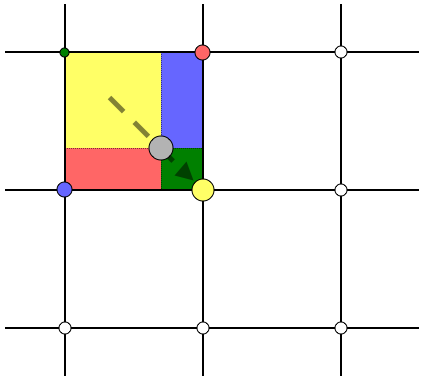
\includegraphics[width=0.8\textwidth]{grid}
\caption{A representation of a two dimensional grid. The particle (grey circle) moves through the domain and deposits charge on the grid points. The area of the rectangle is proportional to the amount of charge deposited at each grid point.\cite{grid}}
\label{fig:grid}
\end{figure}



At the beginning of a PIC simulation the grid is loaded with a particular distribution of particles depending on the plasma parameters to be modelled. It then follows an algorithm as depicted in figure \ref{fig:piccycle}. Each particle deposits charge to neighbouring grid points, Poisson's equation is solved to obtain a potential, the derivative of this is used to calculate the electric field and the field is mapped back to the particles which are then accelerated and moved. Once the particles have been moved, the PIC algorithm is complete, time is advanced by one time step and the whole cycle restarts by calculation of a new charge density based on the updated particle positions. This cycle will carry on until a certain time has been reached or steady-state has been obtained. The aforementioned steps are essential to any application of the PIC method to plasma simulations. Additonal steps can also be added to the cycle based on the requirements of the user. These steps can include Monte Carlo collsions between the particles, absorption and injection of particles and other boundary effects such as sputtering, secondary electron emission and specular reflection. This steps are often added to the end of the PIC cycle once all the original particles in the system have been moved. 

Each step of the PIC cycle will now be detailed. For each of these steps highly optimised algorithms have been developed that are suitable for specific users. For clarity the most general methods will be discussed with specific focus on the algorithms used by VORPAL. 

% The amount of real particles a superparticle represents is labelled the weight of the superparticle. Weights in PIC simulations can vary from $10^3 \rightarrow 10^24$ depending on the plasma to be modelled and the dimensionality of the simulation.

% The use of superparticles makes it feasible to simulate high density plasmas.

%A PIC simulation follows an algorithm that starts with weighting the charge density of particles on to each grid point, typically particles will contribute charge only to the grid points closest to them. Different weighting schemes are possible and will be discussed. Once the charge density has been calculated it is then used to work out the electric potential by solving Poisson's equation. Again the potential is only solved at each grid point. Potential values are now used to calculate electric field values at the grid points which are then interpolated back to the particles, typically using the same weighting as for charge density so that new particle velocities and positions can be determined. Once the particles have been moved, the PIC algorithm is complete, time is advanced by one time step and the whole cycle repeats with a new density being calculated based on the new positions of the particles. This cycle will carry on until a certain time has been reached or steady-state has been obtained. PIC simulations are restricted by the size of the grid cells and the value of the time step as will be explained in more detail.



\begin{figure}[H]
\centering
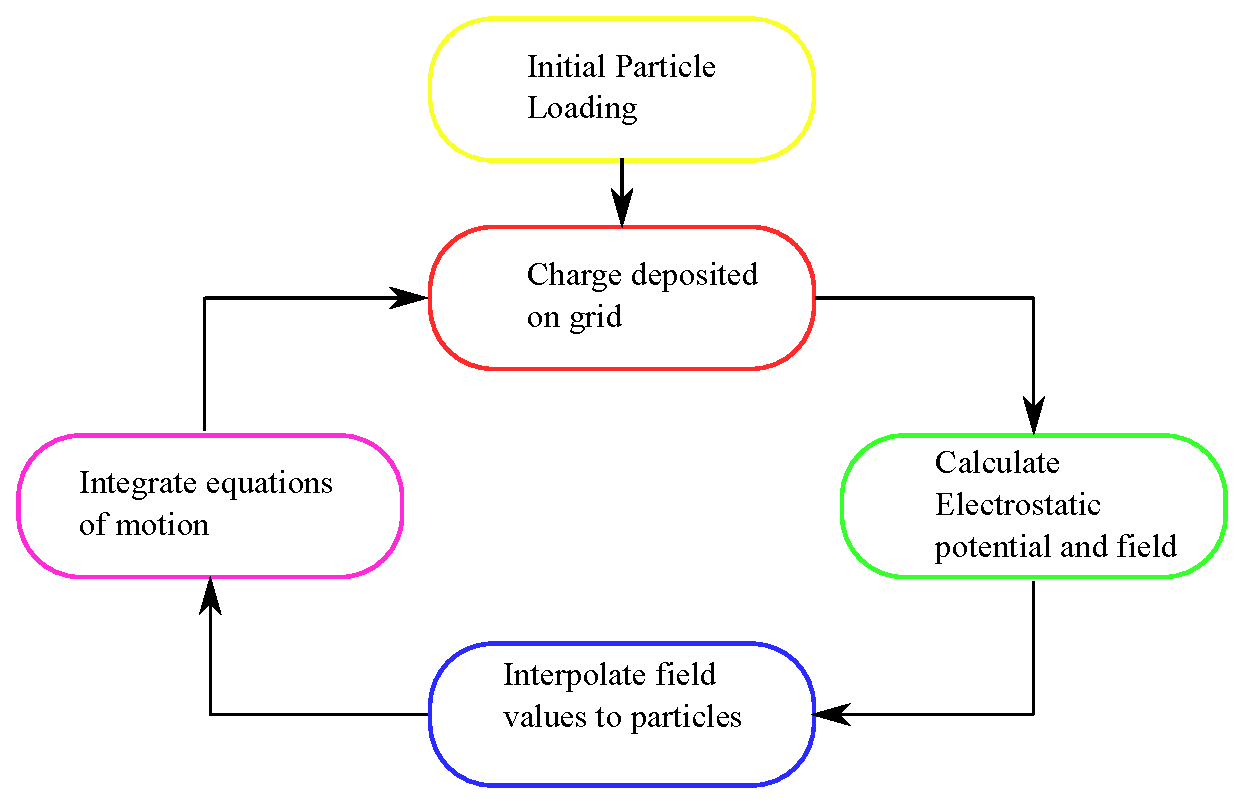
\includegraphics[width=0.8\textwidth]{piccycle.eps}
\caption{A flow chart of the essential steps of the PIC algorithm }
\label{fig:piccycle}
\end{figure}


%"A proper understanding of the sheath phenomena is also an important prerequisite for obtaining boundary conditions for fluid codes simulating tokamaks."
\subsubsection{Calculating the Density}
Weighting is the name given to the calculations which produce charge densities at the grid points from the continous particle positions. Different weighting schemes have been developed and there is often a trade off between accuracy and computation time. The simplest weighting method is the Nearest Grid Point (NGP) scheme. This is a zero order weighting method in which the entirety of the particles charge is assigned to the grid point which it is closest to. Any particles within half a cell of a grid point are assigned to that grid point. Let the cell width be $\Delta x$, $x$ the distance from the grid point and $W(X)$ denote the weighting at grid point $X$. In the NGP scheme 

\be
    W(x)=
    \begin{cases}
      1, & \text{if}\ x \leq \frac{\Delta x }{2}   \\
      0, & \text{otherwise}
    \end{cases}
\ee

This is a computationally fast weighting method as it only requires one grid point look up per particle but this comes at the expense of adding noise to the simulation. As a particle moves away from its original grid point and into the region of a new grid point the grid density at the new grid point suddenly jumps up to have a value of one and the grid point it just left falls down to zero. This weighting scheme is not commonly deployed due to the noisy transition as particles move between cells.  A less noisy method is desired. First-order weighting also known as area weighting smooths the density and field fluctuations compared to NGP but is more computationally expensive as it requires more grid point look-ups for each particle. In this method for a 1D simulation each particle contributes charge to its nearest two grid points. The first step calculates the offset of the particle from the closest grid point to its left. 
\be
offset = x_i - X_j 
\ee 
where $x_i$ is the particles position and $X_j$ the grid point and $x_i > X_j$ always. The charge assigned to the $j^{th}$ grid point is then 
\be 
q_j = q_c \left(1 - offset\right)
\ee 
where $q_c$ is the charge of the particle. 
The charge assigned to the j+1 cell is 
\be 
q_{j+1} = q_c \left(offset\right)
\ee 
This results in a much smoother contribution to the density as the particle moves through the grid. This is the most commonly employed weighting scheme and is the default for VORPAL. Higher order weighting methods do exist such as quadratic and cubic splines, that are second order and third order accurate respectively. These schemes further smooth the non-physical noise at the expense of more computation time by increasing the number of grid points that a particle contributes its charge to. This does lead to problems at the edge of the boundary where there are insufficient neighbouring grid points. 




%Use this for picutre %http://porl2.tripod.com/sitebuildercontent/sitebuilderfiles/mphysproject.pdf
\subsubsection{Calculating the Potential}
Now the charge density is known at each grid point, Poisson's equation for electrostatics can be solved to obtain the electrostatic potential.
\be
\nabla ^2  = -\frac{\rho}{\epsilon_0}
\ee
This can be solved numerically on a discretised grid using the Finite Difference Method (FDM). FDM solves a  differential equation via the discretisation of its derivatives. The first step is to carry out a Taylor series expansion of the potential, first in the forward direction.
\be
\psi(x+\Delta x) = \psi(x) + \Delta x \frac{\partial \psi}{\partial x} + \frac{{(\Delta x)}^2}{2}\frac{{\partial}^2\psi}{\partial x^2} + ...
\label{eq:forward}
\ee
The same procedure can be applied in the backwards direction 
\be
\psi(x-\Delta x) = \psi(x) - \Delta x \frac{\partial \psi}{\partial x} + \frac{{(\Delta x)}^2}{2}\frac{{\partial}^2\psi}{\partial x^2} + ...
\label{eq:backward}
\ee
These two equations can be combined to give an approximate value for the second derivative of potential. Summing \eqref{eq:forward} and \eqref{eq:backward} and rearranging gives 
\be 
\frac{{\partial}^2\psi}{\partial x^2} = \frac{\psi(x+\Delta x) -2\psi(x) + \psi(x-\Delta x)}{{(\Delta x)}^2}
\label{eq:phisolver}
\ee 
In FDM the solution to the equation is only known at the grid points, the potential is no longer a continuous function. Combining the forward difference and backward difference solution like this is known as central differencing and is second order accurate. For clarity we rewrite \eqref{eq:phisolver} with labels based on the grid number $j$. 
\be 
\frac{{\partial}^2\psi}{\partial x^2} = \frac{\psi_{j+1} -2\psi_{j} + \psi_{j-1}}{{(\Delta x)}^2} = -\frac{\rho_j}{\epsilon_0}
\label{eq:phisolver1}
\ee 

The value of $\psi$ at grid point j, ($\psi_j$),  depends on the value of $\psi$ at the two grid points either side of it $(\psi_{j-1}$ and $\psi_{j+1})$, so the grid points are coupled together. In order to find the value of $\psi_j$ at $N$ different grid points requires the solution of $N$ coupled linear equations. These coupled equations can be expressed in matrix form. 
\be
\begin{pmatrix}
  B_{1} & C_{1}  \\
  A_{2} & B_{2} & C_2 \\
        & A_3  & B_3 & C_3   \\
        & & \ddots & \ddots & \ddots \\
        & & &  A_N & B_N
\end{pmatrix}
\begin{pmatrix} 
 \psi_1  \\ 
 \psi_2  \\ 
 \psi_3  \\ 
 \vdots  \\
 \psi_N
\end{pmatrix}
= 
\begin{pmatrix} 
 \rho_1  \\ 
 \rho_2  \\ 
 \rho_3  \\ 
 \vdots  \\
 \rho_N
\end{pmatrix}
\ee
Where $A=1, B=-2$ and $C=1$. A matrix like this with non-zero elements only on the diagonal and one place either side of it is known as a tri-diagonal matrix.  The value of $\rho$ at each grid point is known as it was calculated in the previous step of the PIC algorithm. This matrix equation must now be solved in order to obtain the potential at each grid point. There are various numerical methods to find the solution and they can be divided into two categories: iterative methods and direct methods. Iterative methods begin with an estimate for the solution and use this estimate to get a better estimate. The iterations continue until the error in the estimated solution is below a certain pre-set tolerance. Iterative solves are useful in PIC applications as the potential at the previous time step can be used as the initial estimate for the next time step \cite{poisson_solvers}. Direct methods only need to solve the equation once and do not rely on an initial estimate and so are generally faster in obtaining a solution. They are however harder to implement and more demanding on computer resources. ALSO WHY CAN'T BE USED FOR PARELLEL.
Before a solution can be found the boundary conditions must be supplied as the grid points at the edge of the domain only have one neighbouring grid point. Two common choices for boundary conditions exist, Dirichlet boundary conditions where $\psi_1$ and $\psi_N$ are set to a fixed value or Neumann boundary conditions where the gradient of the potential is fixed at the boundary. 
The implementation of Dirichlet boundary conditions is simple, $B_1$ and $B_N$ are set equal to one and $\psi_1$ and $\psi_N$ are then given the desired potential boundary values $\alpha $ and $\beta$  respectively. The first and last matrix equations then read
\be 
1.\psi_1 + 0.\psi_2 = \alpha 
\ee 
\be 
0.\psi_{N-1} + 1.\psi_N = \beta 
\ee 

Neumann boundary conditions involve fixing the gradient of the potential(i.e. the electric field) at the edge of the domain. This could be implemented by setting $B_1  = -\frac{1}{\Delta x}$, $C_1 = \frac{1}{\Delta x}$ and $\rho_1$ = $\alpha$. Thus giving the first line in the matrix equation as 
\be 
\frac{\psi_2 - \psi_1}{\Delta x} = \alpha 
\ee 

Once the boundary conditions have been supplied the tri-diagonal matrix equation can be solved.
 
%Plenty of tri-diagonal matrix solvers exist including the tridag solver found in Numerical Recipes\cite{NumericalRecipes}.
\subsubsection{Calculating the Electric Field}
MENTION WHY YOU DON't CALCULATE FIELD STRAIGHT AWAY WITHOUT POTENTIAL
Once the potential is known at each grid point the electric field is easily found by calculating the gradient of the potential.
\be 
E = - \nabla \psi
\ee 
which in one dimension becomes
\be 
E = - \frac{\partial \psi}{\partial x}
\label{eq:electricfield}
\ee
This can discretised as before using the central difference method. 
\be 
E_J = - \frac{\psi_{J+1} - \psi_{J-1}}{2 \Delta x}
\ee 
Central differencing is not applicable at the boundaries due to a lack of neighbouring grid points and so either the forward or backward difference method must be used which is only accurate to first order. This provides the following two conditions to calculate the electric field at the edge of the domain.
\be
E_0 = - \frac{\psi_{J+1}-\psi_0}{\Delta x}
\ee 
\be 
E_N = - \frac{\psi_N - \psi_{N-1}}{\Delta x}
\ee
Using a first order equation at the boundaries reduces the accuracy throughout the solution to first order. Fortunately the accuracy can be improved to second order by carrying out a further Taylor expansion 
\be
\psi(x+2\Delta x) = \psi(x) + 2\Delta x \frac{\partial \psi}{\partial x} + \frac{{(2\Delta x)}^2}{2}\frac{{\partial}^2\psi}{\partial x^2} + ...
\label{eq:forward2}
\ee
Combining equations \eqref{eq:forward} , \eqref{eq:forward2} and \eqref{eq:electricfield} gives 
\be 
E_0 = \frac{3\psi_0 + \psi_2 - 4\psi_1}{2\Delta x}
\ee 
The exact same method in the backwards direction gives 
\be 
E_N = \frac{4\psi_{N-1} - \psi_{N-2} - 3\psi_N}{2\Delta x}
\ee
The second order boundary conditions restore second order accuracy across the domain.
\subsubsection{The Particle Mover}
The final step in the PIC cycle is to calculate a new position and velocity for each particle in the simulation based on the forces acting on them. In order to do this Newtons equations of motion must be solved 
\be 
\vec{F}  = m \frac{d \vec{v}}{d t}
\ee 
\be 
\vec{v} = \frac{d \vec{x}}{d t}
\label{eq:diff2}
\ee 

For a particle in an electromagnetic field, the force experienced will be given by the Lorentz force
\be
\vec{F} = q\left[\vec{E} + \vec{v} x \vec{B}\right]
\ee




%Ignoring the presence of a magnetic field for now and limiting to one dimension gives the following equation of motion.
%\be 
%\frac{d \vec{v(x)}}{d t} = \frac{q}{m} E(x)
%\label{eq:diff1}
%\ee

The particles positions and velocities can be found by integrating the differential equations \eqref{eq:diff2} and \eqref{eq:diff1} using finite difference methods. VORPAL uses a leap-frog scheme with a Boris advance to push the particles. 
The leap-frog method involves offsetting the velocity by half a time step from the position. So the velocity of the particles is only known at half integer time steps while the positions are known at integer time steps. This requires the initial velocities of the particles to be moved back half a time step at the beginning of the simulation, a "de-acceleration", in order to have time centred velocities. This just requires calculating the fields as before. This method is known as Leap-frog because in order to calculate new positions requires a leap over the known velocity. 

\begin{figure}[H]
\centering
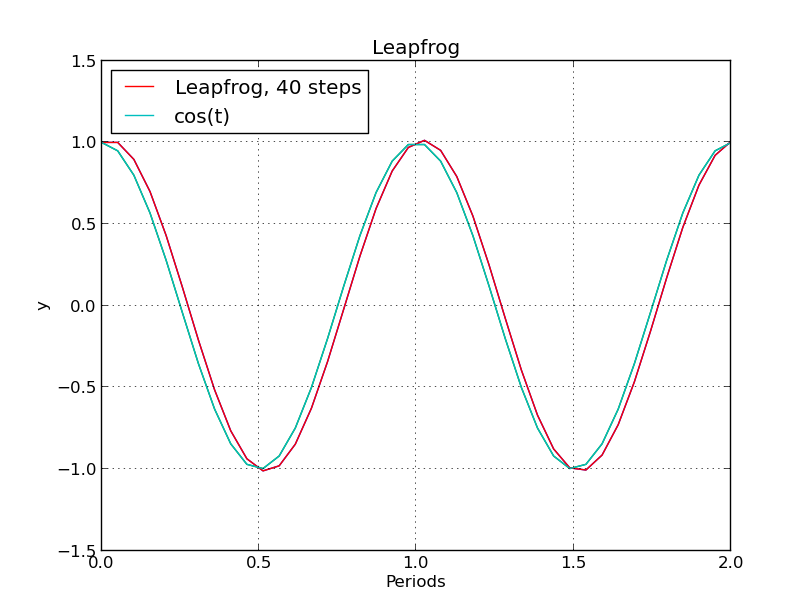
\includegraphics[width=0.8\textwidth]{Leapfrog}
\caption{A graphical representation of the Leap-Frog scheme\cite{shape}}
\label{fig:Leapfrog}
\end{figure}
Instead of using the velocity at time $t$ to move the particle from $t$ to $t+1$ like the Euler method, Leap frog uses the velocity at time $t+\frac{1}{2}$ i.e. the average velocity of the particle between those two times. This method is more accurate than Euler's method for the same computational expense. The only extra step involves pushing back the particles half a time step but this only needs to be carried out once. For this reason Leap-frog is always the preferred choice over Euler and it can be proven to be second order accurate \cite{second_order}.
In discretised form the equations of motion become
\be 
\frac{x_{t+1}-x_t}{\Delta_t} = v_{t+1/2}
\label{eq:new_pos}
\ee
\be
\frac{v_{t+1/2} - v_{t-1/2}}{\Delta_t} = \frac{q}{m}\left[\vec{E_t} + \frac{(v_{t+1/2}+v_{t-1/2}) }{2} x B_t \right]
\label{eq:new_vel}
\ee 
First eqution \ref{eq:new_vel} must be solved to get the new velocity of the particle ($v_{t+1/2}$), this is then inserted into equation \ref{eq:new_pos} to obtain a new position for the particle ($x_{t+1}$). This is carried out for every particle in the system. 


The most common implementation of the Boris scheme seperates the effects of the electric and magnetic fields.
Firstly half of the impulse due to the electric field is added to the particle's velocity creating an intermediate variable $v^-$/
\be
v^- = v_{t-1/2} \frac{q}{m} E_t \frac{\Delta t}{2}
\ee
The magnetic field then acts on $v^-$ to create a second intermediate variable $v^+$. The magnetic field only effects the rotation of the velocity vector not the magnitude.
\be 
\frac{v^+ - v^-}{\Delta t} = \frac{q}{2m} (v^+ + v^-) x B_t
\ee
Finally the second half of the electric impulse is added to $v^+$ to obtain the new velocity for the particle.
\be 
v_{t+1/2} =  v^+ + \frac{q}{m} E_t \frac{\Delta t}{2}
\ee
The Boris scheme can be used to advance particles for an arbitrarily large number of time steps whilst remaining accurate and is therefore the de facto standard for particle movers \cite{boris_good}. 


%\be 
%v_{t+1/2} = v_{t- 1/2} + \frac{qE_t}{m} \Delta t
%\ee
%\be 
%x_{t+1} = x_{t} + v_{t+1/2} \Delta t
%\ee 


% There are many ways in which these equations can be integrated, the methods vary in their complexity to implement as well as run time and accuracy. 
%
%
% Depending on the needs of the simulator, a trade off may need to be made between fast run time and high accuracy. 

%%The simplest method of integration is Euler's method.
%%The finite difference method is used again to discretise the equations. 
%\be 
%v_{t+\Delta t} = v_t + \frac{dv}{dt} \Delta t + \frac{d^2v}{dt^2} {(\Delta t)}^2 + ...
%\ee
%\be 
%x_{t+\Delta t} = x_t + \frac{dx}{dt} \Delta t + \frac{d^2x}{dt^2} {(\Delta t)}^2 + ...
%\ee
%
%In the Euler method The largest term neglected is $\propto {(\Delta t)}^2$. After taking $N$ steps where $N = \frac{total time}{\Delta t}$ the error is now proportional to $\Delta t$. For the case of charged particles moving in an electric field the equations of motion can now be written as
%\be
%v_{t+1} = v_t + \frac{qE}{m} \Delta t
%\label{eq:accelerate}
%\ee
%\be 
%x_{t+1} = x_t + v_t \Delta t
%\label{eq:move}
%\ee 
%The field has been solved already in the previous step of the PIC cycle so $E$ is known. This is then used to accelerate the particle to a new velocity \eqref{eq:accelerate}. The new velocity is then used to find a new position \eqref{eq:move}. All particles are given an initial position and velocity at the start of the simulation so $x_0$ and $v_0$ are known.  The Euler method is very simple to implement and fast to run but is only first order accurate.
%
%To demonstrate the stability of the Euler method it will now be applied to the case of a mass on a spring with equation of motion 
%\be 
%\frac{d^2 x}{dt^2} = -\frac{k}{m} x 
%\ee
%where $k$ is the Stiffness constant of the spring and $m$ is the mass of the attached object. An initial value for the position and velocity is required e.g. $v=1, x=0$.  Euler's method would approximate the equations of motion as 
%\be
%v_{t+1} = v_t - \frac{k}{m} x \Delta t 
%\ee
%\be 
%x_{t+1} = x_t + v_t \Delta t
%\ee
%These equations can be solved multiple times to advance the system from its initial state. To check the accuracy of the Euler method the results are compared to the known analytical solution. 
%\begin{figure}[H]
%\centering
%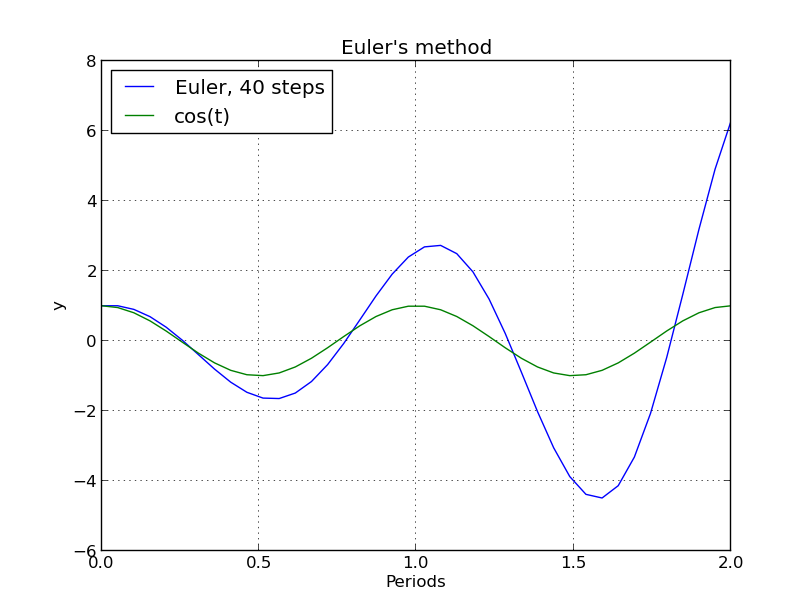
\includegraphics[width=0.8\textwidth]{Euler}
%\caption{Euler solution to harmonic oscillator compared to analytical solution.}
%\label{fig:E}
%\end{figure}
%The Euler method is unstable and quickly diverges from the analytical solution. This is no surprise based on the simplicity of the method. A more stable, higher order accurate integrator is desired for use in PIC codes.  Euler's method is described as an Explicit method as it uses the state of the system at the current time step to advance the system to its next time state. Implicit methods on the other hand use both the state of the system at the current time and the state of the system at the next time step to evolve the state of the system. An example of this is the Backwards Euler method. In this case the value of the velocity at time $t$ can be expressed as 
%\be
%v_t = v_{t+1 -\Delta t} = v_{t+1} - \Delta t \frac{dy}{dt}\Bigr|_{\substack{t=t+1}}
%\ee
%using a backwards Taylor expansion. Rearranging gives 
%\be 
%v_{t+1} = v_t +  \Delta t \frac{dy}{dt}\Bigr|_{\substack{t=t+1}} 
%\ee 
%A similar expression is found by replacing $v$ with $x$. Applying this to the case of the simple harmonic oscillator 
%\be 
%v_{t+1} = v_t - \Delta t\frac{k}{m} x_{t+1} 
%\ee 
%\be 
%x_{t+1} = x_t - \Delta t\frac{k}{m} v_{t+1} 
%\ee
%The new value of the variable no longer depends on two known values as in the case of the Euler method but now depends on an unknown value from the next time step. It can be solved using the Newton-Raphson method. Implicit schemes are stable but more computationally expensive, this can be offset by the fact they allow for larger time steps to be taken and so can evolve a system to a desired time using less time steps than an explicit scheme. The stability of the numerical methods is not the only thing that limits the size of the time step in PIC codes, the size of the timestep is limited by the natural frequencies of the system \cite{Hockney1981}. This will be discussed more in the practical considerations section. The computational expensive and the need to use small time steps often rules out the use of implicit methods for the particle mover of PIC codes. 
%
%
%Fortunately a more stable, explicit  method exists that is very similar to the Euler method and requires the same number of computations per time step but also has the advantage of being second order accurate. The Leapfrog method expands upon the Euler method. Instead of using the velocity at the beginning of the time step to advance the position it uses an average value of velocity throughout the time step. The leap-frog method involves offsetting the velocity by half a time step from the position. So the velocity of the particles is only known at half integer time steps while the positions are known at integer time steps. 
%\be 
%v_{t+1/2} = v_{t- 1/2} + \frac{qE_t}{m} \Delta t
%\ee
%\be 
%x_{t+1} = x_{t} + v_{t+1/2} \Delta t
%\ee 
%This requires the initial velocities of the particles to be moved back half a time step at the beginning of the simulation, a "de-acceleration", in order to have time centred velocities. This just requires calculating the fields as before. This method is known as Leap-frog because in order to calculate new positions requires a leap over the known velocity. 
%
%\begin{figure}[H]
%\centering
%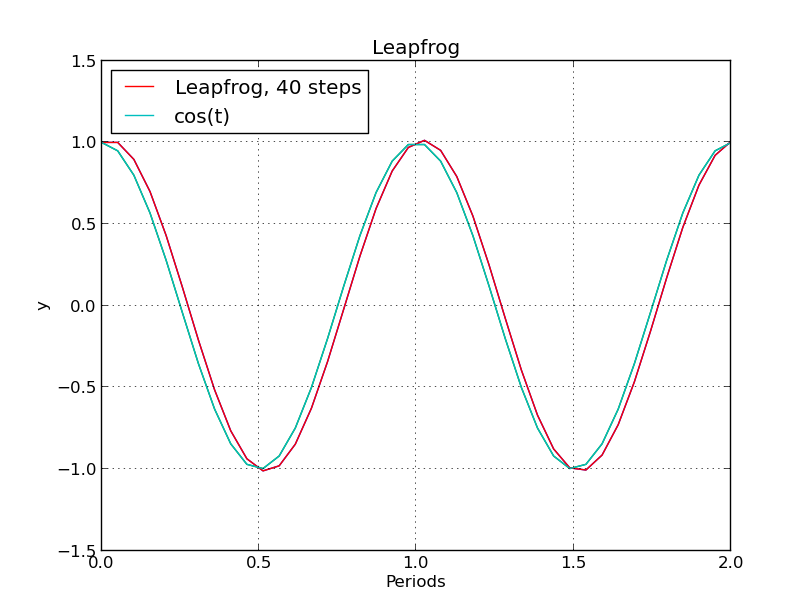
\includegraphics[width=0.8\textwidth]{Leapfrog}
%\caption{A graphical representation of the Leap-Frog scheme\cite{shape}}
%\label{fig:Leapfrog}
%\end{figure}
%Instead of using the velocity at time $t$ to move the particle from $t$ to $t+1$ like the Euler method, Leap frog uses the velocity at time $t+\frac{1}{2}$ i.e. the average velocity of the particle between those two times. This method is more accurate than Euler's method for the same computational expense. The only extra step involves pushing back the particles half a time step but this only needs to be carried out once. For this reason Leap-frog is always the preferred choice over Euler and it can be proven to be second order accurate \cite{second_order}.
%This method can also be applied to the case of the mass on a spring as before and compared to the analytical solution.
%\begin{figure}[H]
%\centering
%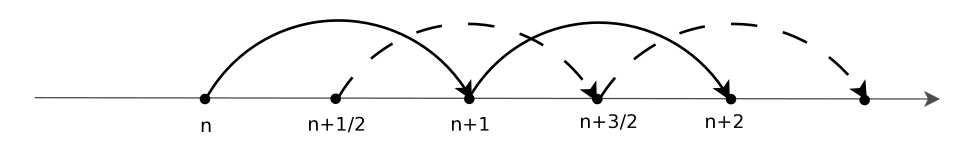
\includegraphics[width=0.8\textwidth]{leapfrog}
%\caption{A comparison of the numerical solution to the problem of a mass on a spring using the leapfrog method compared to the analytical solution.}
%\end{figure}
%This was run with as many time steps as Euler. It is clearly more stable. As with all explicit methods there exists a critical time step size, exceeding this leads to numerical instabilities. In the case of leapfrog $w dt <2 $ where $w$ is the highest frequency in the problem, usually the electron plasma frequency. COULD PROVE THIS WITH THE HARMONIC OSCILLATOR. However as mentioned before there are other factors which force the time step to be small for PIC codes so this is not a disadvantage to the Leap Frog method.
\subsubsection{Stability Conditions}
%explicit methods have regirous time constraints for stability condtions. THEN IMPLICIT METHODS EXIST that aim to increase the length of the time step while remaining stable e.g. cite the thesis I'm reading. Then mention why these aren't used.

PIC simulations utilise FDEs to find solutions to continous differential equations on a discretised grid. The use of FDEs can provide accurate physical results provided three stability conditions are met. The first places a constraint on the size of each grid cell ($\Delta x$). 
\be
\Delta x < \frac{\lambda_D}{0.3}
\ee
PIC codes can only resolve phenomena that are larger than $\Delta x$, anything smaller than this is smoothed over. PIC codes must resolve the Debye length in order to accurately capture the shielding effects. The second constraint is that the plasma frequency must be resolved meaning that
\be
\Delta t < \frac{2}{\omega_p}
\ee
The time step is further contrained by the criteria that no particle should be able to travel more than one grid cell in a given time step. 
\be 
\Delta t < \frac{\Delta x}{v_{max}}
\ee
where $v_{max}$ is the speed of the fastest moving particle in the system. For high density, low temperature plasmas $\lambda_D \approx 10^{-6}$ while electron velocities can exceed $10^6 ms^{-1}$. This means thousands of grid cells may be necessary to simulate the $10mm^2$ tip of a Langmuir probe with time steps as small as $10^{-12}s$. Simulations with these demands can only be carried out on supercomputers.

%"Despite having many advantages, the PIC model also has a number of weaknesses. Perhaps
%the most quickly encountered of these is computational efficiency. This is a consequence of
%the statistical model in which numerical fluctuations converge as N−1/2 for N particles; the
%PIC scheme and some modifications can reduce the constant but not the scaling. An associated
%problem is the difficulty in resolving the tail of the distribution, which is often poorly populated
%by statistical methods. It is also challenging to model large ranges of timescales, as short
%timescales require small time steps while long timescales require running many time steps.
%Similarly, large ranges of space scales present similar difficulties for the mesh size. Finally,
%the PIC method requires significant memory and processor resources, and for the foreseeable
%future this will remain the case. Fortunately, the boundaries of what is possible are always
%advancing by virtue of Moore’s law and new algorithms"
%
%"Strict requirements on the spatio-temporal spacing in explicit PIC scheme put constraints on the time
%scales that this method can successfully address. On the other hand it is a very powerful method which
%easily allows for including many additional physical phenomena, such as collisions, production and loss
%of particles, or interaction with solid surfaces."

\subsubsection{Consequences of Using a Grid}
This gives the particle an effective shape, in this case rectangular. The particle also has a finite size of width $\Delta x$. Finite sized particles are a direct result of weighting particles on to the grid. The weighting method determines the effective size and shape of the particle as viewed by grid. Due to the large jumps to grid values caused by the movement of particles from one grid point to the next, the NGP weighting method is a large source of noise in the density and field calculations.
The weighting puts the fraction of the clouds charge which is in the $J^{th}$ cell to the $X_J$ grid point and the rest of it goes to the $X_{J+1}$ grid point. This  gives the particle a triangular shape, so the particle is effectively a triangular cloud of uniform charge centred at $x_i$ with a width of $2\Delta x$ as it is able to influence a grid point from both sides of it.
\begin{figure}[H]
\centering
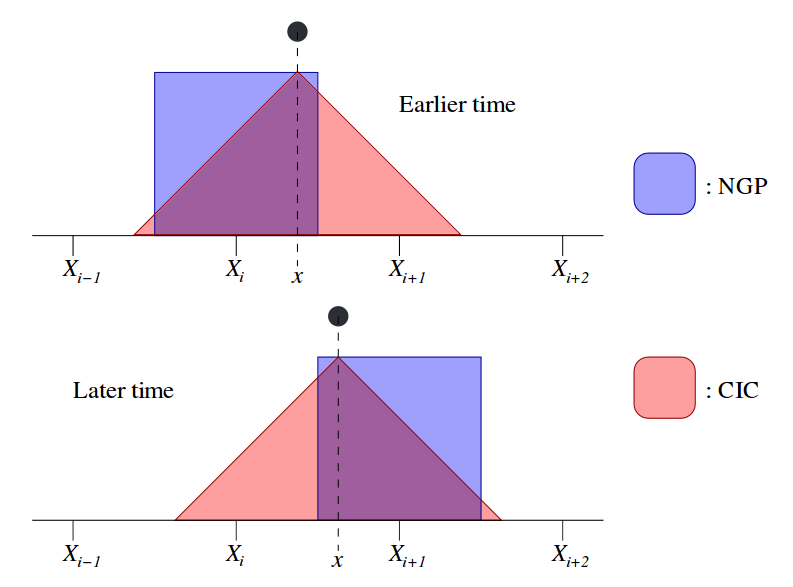
\includegraphics[width=0.8\textwidth]{particleshape}
\caption{The effective shape of a particle at position x as seen by the grid.\cite{shape}}
\label{fig:shape}
\end{figure}


\subsubsection{Particle Injection}
In Langmuir probe simulations, particles are lost to the various collecting surfaces and must be replaced so that a constant density plasma can be simulated. It is therefore neccessary to include an additional step of particle injection into the PIC alogirthm. Particle injection takes place at the end of the PIC cycle once all other particles have been moved.
It is desirable to inject particles at a rate that conserves the plasma density specified at the beginning of the simulation however it is not a neccessity. The simulation will reach a steady-state density once the particle injection rate is balanced by the outflow rate of particles. The rate required to maintain a constant density plasma can be estimated as 
\be
R_{constant-density} = v_{th,s}\Delta T * N / \Delta x
\ee
where $v_{th,s}$ is the thermal velocity of the species, $\Delta T$ the size of the time step, $N$ the number of particles per cell specified at the beginning of the simulation and $Delta x$ the gridspacing. 

Langmuir probe theory is based on the assumption of Maxwellian velocity distributions an example of which is shown below. At the beginning of the simulation each species can be given a Maxwellian distribution and there exists various algorithms to implement this e.g. birdsall. The simulation will be required to run for many thousands of time steps in order to reach a steady state solution and conserving this distribution over the time required is not so simple. PIC simulations model a small region of the plasma and use superparticles to sample the velocity distribution. As there are orders of magnitude differences between the number of superparticles followed and the true number of particles in a real plasma, losses of superparticles in a PIC simulation can dramatically change the velocity distrubution at very short time scales. The problem is enhanced by the lack of collisions in fusion-relevant PIC simulations. Due to the high densities and low temperatures of a SOL plasma, PIC simulations can only feasible sample small regions of the plasma. The dimensions of the simulation region are often smaller than any collsion mean free paths, so particles are able to move across the whole domain without colliding. Collisions drive particles towards Maxwellian distributions. It is therefore of crucial importance to sample from the correct velocity distribution when injecting particles into the simulation domain. 
In early simulations, particle loading at the beginning of the simulation and particle injection throughout the simulation both used the same source function. For every particle a random velocity was chosen sampled from a Maxwellian distribution. However it was found in practise that this did not conserve the Maxwellian distribution. With increasing simulation time, the velocity distribution of the particles narrowed, resulting in a 'cooling' of the plasma. Get picture of before and after. Although not anticipated the reasons for this are simple. Particles are initially loaded into the simulation domain with a range of velocities all sampled from a Maxwellian distribution. Provided there are enough superparticles in the domain, the distribution will be sufficiently represented by the finite number of particles. As time advances particles exit the simulation once they reach an absorbing boundary layer and new particles enter in the injection phase of the PIC cycle. The fastest particles in the simulation are on average the first to leave as they quickly move across the domain to an absorbing surface. However if the injected particles are also sampled from the same Maxwellian distribution then it is far likely that the injected particle will have a velocity close to zero rather than a high velocity in the tail of the distribution. As a result the fastest particles leave the simulation quickly to be replaced by slow moving particles that hang around for a long time. This results in the fastest particles being under-represented in the simulation. The tail disappears, the distribution narrows and the effective temperature of the plasma cools. Ideal probe theory assumes a constant temperature, Maxwellian plasma. Experimental measurements work on this basis too. It is not possible to compare experimental data with simulation results if the the simulation plasma is not at a constant temperature. A source function that conserves temperature as the simulation runs is desired. This source function must replace the particles at a rate proportional to their velocity. The fastest particles are required to be replaced more often while the slow moving particles not so much. Rather than the Maxwellian distribution that peaks at $v=0$ the new distribution must fall to zero at this point as those particles should never leave the simulation. A method to investigate the shape of the source function was established.
COPY REPORT BIT ON GETTING THE RIGHT SOURCE FUNCTION 
For the purposes of investigating the correct source function to use a 1D simulation was adequate. The simulation domain is shown below.
\begin{figure}[H]
\centering
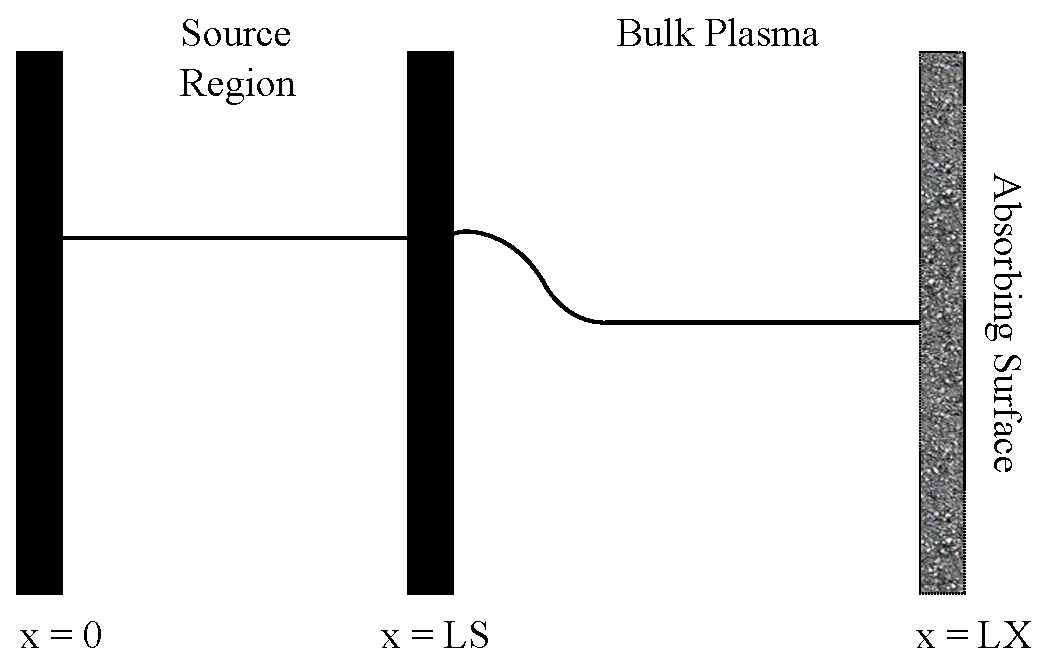
\includegraphics[height=7cm,width=0.8\textwidth]{cloned_source.eps}
\caption{A source region on the left-hand side replaces particles that are lost to the wall.}
\end{figure}
The model tracks a length of plasma , hundreds of Debye Length ($\lambda_D$) long and follows the motion of all ions and electrons as they move in self-consistent electric fields. The presence of a magnetic field  impacts the source function so to begin with only electrostatic simulations were carried out. On one side of the domain is an absorbing surface that represents the probe, any potential can be set to this surface and any charged particles that hit the surface are deleted from the simulation and their current recorded. On the opposite side of the domain is a source region of plasma. The purpose of this source region is to supply the bulk plasma with new particles to replenish those lost to the sides. At the beginning of the simulation a quasi-neutral plasma with a Maxwellian distribution fills the entire domain. Any particles born into the source region ($0\leq x \leq LS$) are trapped in the source region for the duration of the simulation. These source particles travel back and forth in the source region and are reflected at the boundries $x=0$ and $x=LS$. Both edges of the source are held at the same potential ($V_{source}$) which fixes the plasma potential. As there is no potential difference between the two sides and no particles can escape the plasma source remains at the temperature and density specified at the beginning of the simulation. The plasma maintains the Maxwellian distribution throughoutthe simulation as shown in figure \ref{fig:maxwell_maintained}.
\begin{figure}[H]
\centering
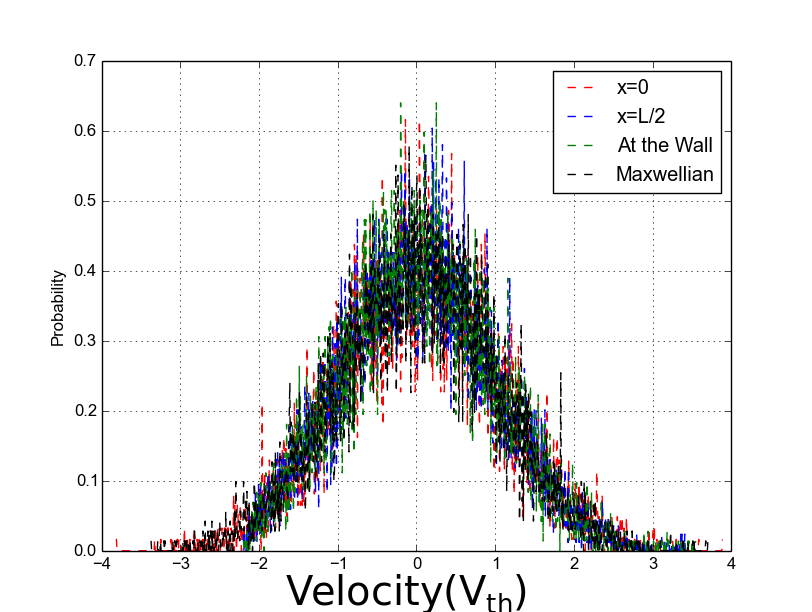
\includegraphics[height=7cm,width=0.8\textwidth]{maxwell_maintained.png}
\caption{The velocity distribution of particles in different regions of the plasma at the end of the simulation. The Maxwellian distribution is conserved.}
\label{fig:maxwell_maintained}
\end{figure}
Any source particle striking the $x=LS$ boundary is copied before being reflected. This copy is identical to the original particle, having the same charge, mass, position and velocity but is not reflected at the boundary. Instead the copy travels into the bulk plasma, allowing the source region to replenish the plasma. By looking at the velocity distribution of particles exiting the source it is possible to determine the form of the source function required to sample a Maxwellian plasma. The distribution of particles leaving the source region is equivalent to the distribution of particles that would exit the simulation of a bulk plasma. It is these velocities that must be sampled in order to maintain a constant temperature plasma. The velocity distribution of particles leaving the source is shown below.
GET EMMERT PLOT
Describe the plot, cite Emmert paper and the source function.

As well as providing a source function this method provided validation for the rate of injection. It was found that the ratio of electrons exiting the source to ions exiting the source was equal to the ratio of their thermal velocities. Now a temperature conserving source function has been determined there is no need for the source region. Simulating the source region requires tracking many particles, which is feasible in 1D simulations but would take up too much time for higher dimensions. The simulation domain now looks like this.
\ref{fig:maxwell_maintained}.
\begin{figure}[H]
\centering
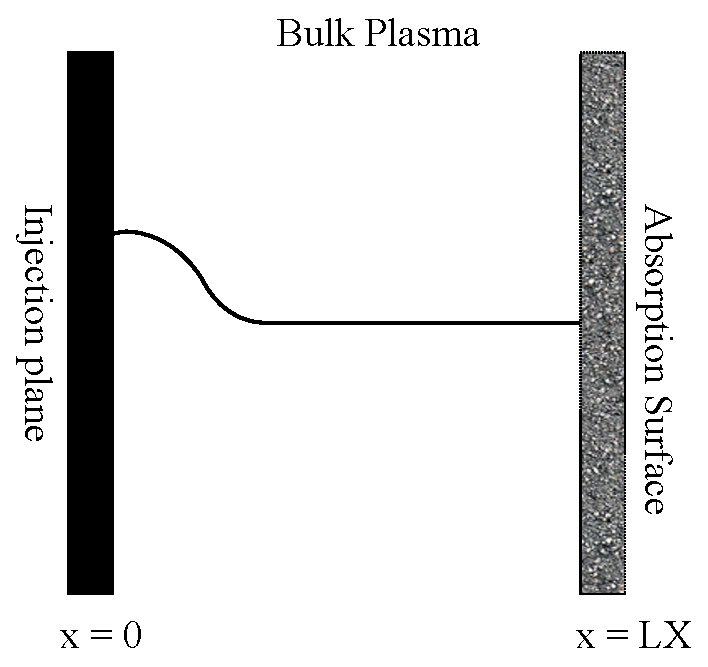
\includegraphics[height=7cm,width=0.8\textwidth]{ideal_probe_test.eps}
\caption{The velocity distribution of particles in different regions of the plasma at the end of the simulation. The Maxwellian distribution is conserved.}
\label{fig:maxwell_maintained}
\end{figure}




    A plasma source is required to replenish particles that are lost to the probe. This source can be held at any potential, I choose 0V, this sets the plasma potential. The system reaches a steady state over a few ion transit times at which point the current drained by the probe surface reaches a constant value and the plasma density stabilises. The domain is shown below. 
%For the IOP conference I wanted to produce probe IV curves from my simulations and then apply ideal probe theory to the IV curve to see if I could measure the plasma temperature and density. In essence treating the simulation measurements in the same way as experimental data. Ideal probe theory assumes no magnetic fields, collisions or plasma-surface interactions, so if I set my simulations up without these effects I should be able to reproduce the fundamental prediction of ideal probe theory - the electron current drops off exponentially as the probe is biased more negatively with respect to the plasma potential, this is expressed in equation \eqref{e_falloff}. 
%\be
%\label{e_falloff}
%I_{e} = I_{e,sat} e^{-\frac{V_{probe}}{T_e}}
%\ee
%Where $V_{probe}$ is the bias applied to the probe relative to the plasma, $T_e$ the electron temperature in eV and $I_{e,sat}$ the electron saturation current. This is the electron current the probe would collect if $V_{probe} \geq 0$. This can be rearranged to simplify the measurement of $T_e$.
%\be 
%\ln(I_e) = \frac{V_{probe}}{T_e} + \ln(I_{e,sat})
%\ee
%By plotting the natural logarithm of the electron current against the probe bias and measuring the gradient it is possible to measure the electron temperature. 
%
%
%\subsection{The Simulation Model}
%All results presented here were obtained during the VORPAL trial period using a single core license. The simulations were carried out in 1D. The model tracks a length of plasma , hundreds of Debye Length ($\lambda_D$) long and follows the motion of all ions and electrons as they move in self-consistent electric fields. On one side of the domain is an absorbing surface that represents the probe, any potential can be set to this surface and any charged particles that hit the surface are deleted from the simulation and their current recorded. On the opposite side of the domain is another surface that represents the plasma source. A plasma source is required to replenish particles that are lost to the probe. This source can be held at any potential, I choose 0V, this sets the plasma potential. The system reaches a steady state over a few ion transit times at which point the current drained by the probe surface reaches a constant value and the plasma density stabilises. The domain is shown below. 
%% The simulations however, already have the perfect diagnostic as the position and velocity of all particles is known. This means I can 
% 
%
%\begin{figure}[H]
%\centering
%\includegraphics[height=7cm,width=0.8\textwidth]{IOP_model.PNG}
%\caption{A source region on the left-hand side replaces particles that are lost to the wall.}
%\end{figure}
%
%At the start of the simulation the domain is filled with a uniform density, quasi-neutral plasma. The particles are given a velocity randomly generated from a Maxwellian distribution as shown in figure \ref{maxwell}. For a given run the probe will be biased to a potential and then run until steady state. Completing multiple runs at different bias voltages allows a probe IV curve to be constructed. Simulations were only run in the ion collection region as this is the area of interest in fusion experiments. As mentioned at the end of my first year report this model has a problem with temperature conservation due to the injection of particles to replace those lost to the probe. In my initial attempt to replace lost particles I simply injected new particles with velocities again sampled from a Maxwellian distribution. However, the faster a particle is, the quicker it will be lost to the wall. Due to the nature of a Maxwellian distribution, it is far more likely that the newly injected particle will have a low velocity close to zero and so naturally the high energy tail of the distribution is lost over time. This presents a problem when attempting to apply ideal probe theory to my simulation results. $T_e$ is not a constant in my simulations and varies with $V_{probe}$. As a result each run with a certain $V_{probe}$ sits on it's own IV curve and cannot be compared to the other runs. I needed a source function that only replaced the fast particles lost to the wall and not the zero velocity particles that didn't leave the simulation. It was not obvious what that source function should be, however, I did have another method to get around this.
%\begin{figure}[H]
%\centering
%\includegraphics[height=7cm,width=0.8\textwidth]{maxwellian.PNG}
%\label{maxwell}
%\caption{The initial velocity distribution of particles in the simulation. A particle's velocity is sampled from a Maxwellian distribution.}
%\end{figure}
%
%\subsection{Improvements to the Model}
%In the improved model I did away with the source function altogether. Half way across the simulation I placed a surface that reflected any particles that hit it coming from the left and absorbed any particles that hit it coming from the right hand side. Particles that were born on the LHS of the simulation were trapped by this reflecting plane and would travel back and forth throughout the simulation. The plasma on the LHS conserved the temperature and density specified at the beginning of the simulation, this didn't change over time. I was then able to turn this reflecting region into a source for my simulations. Just before a particle hit the reflecting plane, a clone was made of the particle with the same velocity. This clone was allowed to pass through the reflecting surface and travel to the probe on the right hand side while the original particle was reflected and travelled back towards the left hand side of the domain. I now had a particle source that only replaced particles that should have been able to escape the domain and so replaced the high energy tail lost to the wall. I was able to use this reflecting and cloning source method to reproduce ideal probe theory.
%
%\subsection{Results}
%By recording the electron current drained by the probe in steady state for different probe biases I was able to produce the following graph. 
%
%\begin{figure}[H]
%\centering
%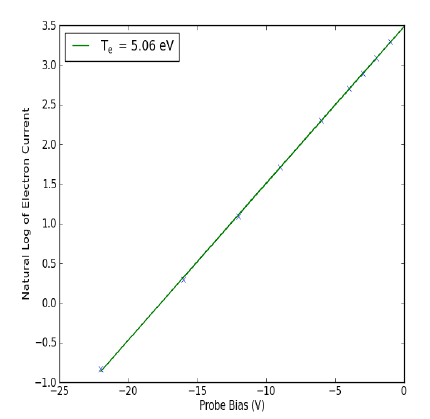
\includegraphics[height=7cm,width=0.8\textwidth]{e_grad.PNG}
%\label{maxwell}
%\caption{The gradient of the natural log plot is equivalent to the reciprocal of the electron temperature.}
%\end{figure}
%
%By measuring the gradient I was able to determine the temperature of the source plasma in the reflecting region. This was repeated for different initial temperatures and always determined the correct result. 
%
%I was also able to produce a probe IV curve in the ion collection regime which agreed well with the theoretical prediction of equation \ref{theoretical}. 
%
%\be
%\label{theoretical} 
%I_{total} = I_{sat} (1 - e^ {(V_{probe} - V_{float})/T_e})
%\ee
%\begin{figure}[H]
%\centering
%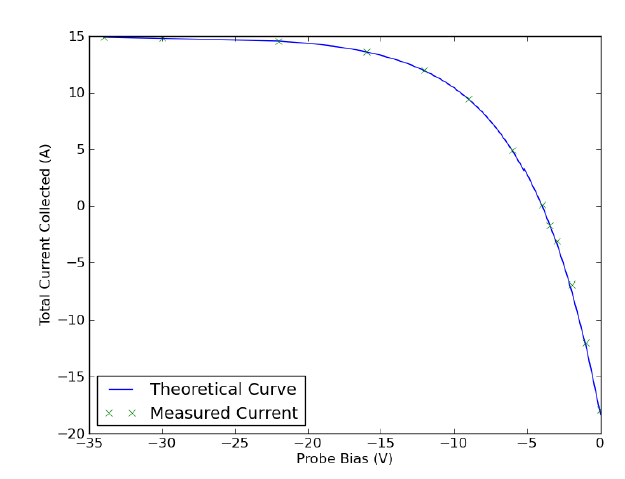
\includegraphics[height=7cm,width=0.8\textwidth]{IV_curve.PNG}
%\label{maxwell}
%\caption{Plot of the probe IV curve in the ion collection region compared to the theoretical prediction. }
%\end{figure}
%
%The ability to reproduce ideal probe theory was a crucial starting point before going on to investigate more realistic scenarios. 





EFFECTS OF ADDING A B FIELD, YOU WANT TO SPECIFY THE PARALLEL VELOCITY BUT HOW TO DO YOU DO THAT WHEN THE FIELD IS TILTED
DETAIL TEST CARRIED OUT TO SHOW PARTICLES MOVES AT CORRECT RATE

 



\chapter{A Chapter} % Write in your own chapter title
\label{Chapter4}
\lhead{Chapter 4. \emph{A Chapter}} % Write in your own chapter title to set the page header


 



\chapter{A Chapter} % Write in your own chapter title
\label{Chapter5}
\lhead{Chapter 5. \emph{A Chapter}} % Write in your own chapter title to set the page header


 



\chapter{A Chapter} % Write in your own chapter title
\label{Chapter6}
\lhead{Chapter 6. \emph{A Chapter}} % Write in your own chapter title to set the page header


 



%% ----------------------------------------------------------------
% Now begin the Appendices, including them as separate files

\addtocontents{toc}{\vspace{2em}} % Add a gap in the Contents, for aesthetics

\appendix % Cue to tell LaTeX that the following 'chapters' are Appendices

% \input{./Appendices/appendixA}	% Appendix Title

%\input{./Appendices/appendixB} % Appendix Title

%\input{./Appendices/appendixC} % Appendix Title

\addtocontents{toc}{\vspace{2em}}  % Add a gap in the Contents, for aesthetics
\backmatter

%% ----------------------------------------------------------------
\label{Bibliography}
\lhead{\emph{Bibliography}}  % Change the left side page header to "Bibliography"
\bibliographystyle{amsplain}
% \bibliographystyle{unsrtnat}  % Use the "unsrtnat" BibTeX style for formatting the Bibliography
\bibliography{Thesis}  % The references (bibliography) information are stored in the file named "Thesis.bib"

\end{document}  % The End
%% ----------------------------------------------------------------